\definecolor{greenish}{RGB}{0,145,0}
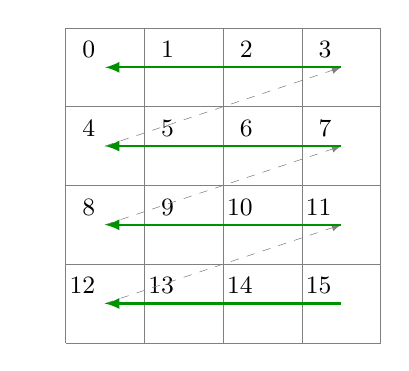
\begin{tikzpicture}[scale=1]
\def \xmax{4}
\def \ymax{4}
\draw[style=help lines, ystep=1, xstep=1]
	(0,0) grid (\xmax,\ymax);

\foreach \y in {0.5,1.5,...,\ymax}
{%
    \foreach \x in {0.5,1.5,...,\xmax}
    {%
      % floor the positions, as they are .5 and reverse vertical order
      \pgfmathtruncatemacro{\posX}{\x}
      \pgfmathtruncatemacro{\posY}{\ymax-\y}
      % calculate the index for each position
      \pgfmathtruncatemacro{\index}{\posX + \xmax * \posY}
      \node[above left] at (\x,\y){\small$\quad\;\index$};
    }
}

\def\startx{0.5}
\def\starty{3.5}

% help lines
\draw[-latex,style=help lines, dashed] (\startx + 0,\starty - 1) --++ (3,1);
\draw[-latex,style=help lines, dashed] (\startx + 0,\starty - 2) --++ (3,1);
\draw[-latex,style=help lines, dashed] (\startx + 0,\starty - 3) --++ (3,1);

% scanning
\draw[latex-,greenish,thick] (\startx,\starty - 0) --++ ( 3,0);
\draw[latex-,greenish,thick] (\startx,\starty - 1) --++ ( 3,0);
\draw[latex-,greenish,thick] (\startx,\starty - 2) --++ ( 3,0);
\draw[latex-,greenish,thick] (\startx,\starty - 3) --++ ( 3,0);

\end{tikzpicture}
